\documentclass{article}

\usepackage{graphicx}
\usepackage{subcaption}
\usepackage[utf8]{inputenc}
\usepackage{amsmath}
\usepackage{float}
\setlength{\parindent}{3em}
\usepackage[a4paper,left=2.5cm,right=2.5cm,top=2.5cm,bottom=3.0cm]{geometry}

\def\bkRsf{{\sf \mbox{\vrule height0.705em width0.06em
            depth0em}\kern-.04em R}}

\renewcommand*\contentsname{Sumário}
\renewcommand{\figurename}{Figura}

\begin{document}

\begin{titlepage}
    \begin{center}
        \large
        \textbf{} MINISTÉRIO DA DEFESA\\
        \textbf{}DEPARTAMENTO DE CIÊNCIA E TECNOLOGIA\\
        \textbf{}INSTITUTO MILITAR DE ENGENHARIA\\
        \textbf{} \textit{}(Real Academia de Artilharia, Fortificação e Desenho - 1792)\\
        \vspace{0.5cm}
 
        \vfill
        
\includegraphics[width=0.4\textwidth]{ime.jpg}

        \vspace{0,9cm}

        \LARGE
        \textbf{Álgebra Linear na Construção da Arquitetura de Controle de Robôs Autônomos com Rodas Omnidirecionais}
 
        \vspace{1,5cm}
        \large
 
        \vspace{2,5cm}
 
        Alexandre Pereira de Freitas\\
        Lucas Rafael de Aguiar Silva\\
        Samuel Morais Barros\\
        Sérgio Reinier Sousa Macário\\
        Vinícius de Freitas Lima Moraes\\
 
        \vfill
 
        \vspace{0.5cm}
 
        \Large
        08/11/2019
 
    \end{center}
\end{titlepage}

\tableofcontents
\newpage

\section{Introdução}
\subsection{Constituição dos robôs com rodas omnidirecionais}

\hspace{1cm} Robôs com movimentação omnidirecional são máquinas capazes de se locomover em todas as direções e ângulos sem a necessidade de rotacionar o seu corpo antes de executar a translação. As peças especiais que permitem isso são as omnirodas, rodas constituídas por várias rodas menores perpendiculares em relação ao plano da roda maior encaixadas ao longo de sua periféria, conforme a figura 1 a seguir:

\begin{figure}[H]
\centering
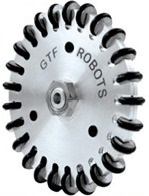
\includegraphics[width=0.4\textwidth]{omniroda.jpeg}
\caption{Omniroda}
\label{Figura 1}
\end{figure}

O princípio de funcionamento dos robôs com omnirodas constitui-se do fato de que, enquanto a roda principal provê tração na direção normal ao eixo do motor, as rodas menores que constituem a roda principal permitem o deslizamento sem atrito (para um estudo ideal) na direção do eixo do motor.\\ \\

\begin{figure}[H]
\centering
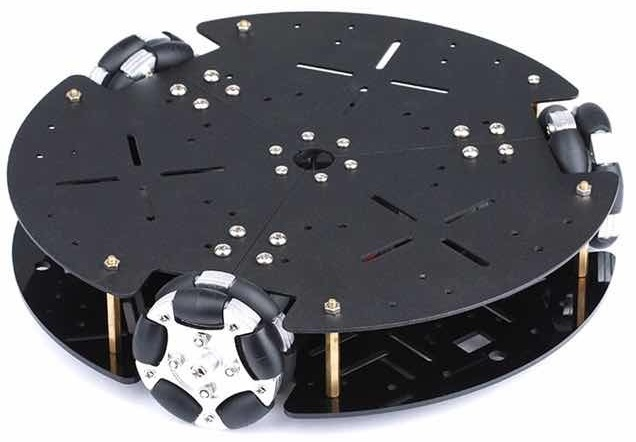
\includegraphics[width=0.4\textwidth]{robo.jpeg}
\caption{Robô com rodas omnidirecionais}
\label{Rotulo}
\end{figure}


Em geral, utiliza-se três ou quatro rodas omnidirecionais na fabricação de um robô, conforme a figura 2. A composição da tração de cada uma das rodas possibilita a translação e a rotação do robô. O ideal seria utilizar duas rodas omnidirecionais ortogonais, de tal forma que somente a translação fosse permitida, minimizando a complexidade do movimento. Porém, por questões espaciais e de estabilidade, esse arranjo é impossível. 
Nesse ínterim, o ideal das rodas omnidirecionais constitui da busca pela situação na qual as $n$ rodas empregadas em um robô possibilitam a obtenção da maior velocidade pelo robô com a maior eficiência energética no sentido desejado.


\subsection{Fundamentos Físicos}

\hspace{1cm}Para a compreensão do movimento, é necessário analisar tanto a translação quanto a rotação do sistema de acordo com a geometria do robô. Para isso, pode-se modelar o robô dotado de $n$ rodas, tal que:

\begin{figure}[H]
\centering
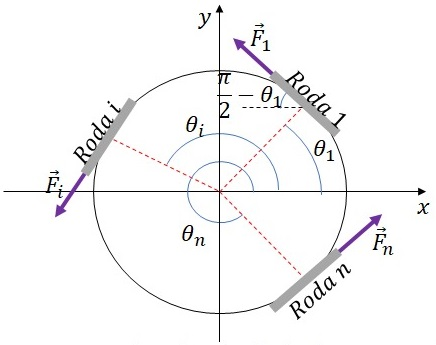
\includegraphics[width=0.4\textwidth]{roda.jpeg}
\caption{Arranjo de $n$ rodas e as aplicadas forças correspondente}
\label{Rotulo}
\end{figure}

Para a translação, pode-se aplicar a 2º lei de Newton com relação ao centro do robô:
\[\vec{F}_{resultante} = M\vec{a}_{resultante}\]
\[\vec{a}=\frac{1}{M}\sum_{i=1}^{n}\vec{F}_i\]
\hspace{1cm}Observa-se, por decomposição vetorial, que:
\[a_x=-\frac{1}{M}\sum_{i=1}^{n}F_i\sin\theta_i \text{ (I)}  \]     
\[a_y=\frac{1}{M}\sum_{i=1}^{n}F_i\cos\theta_i \text{ (II)}\]	
\hspace{1cm}Para a rotação, deve-se analisar o torque resultante:
\[\tau_{resultante}=I\dot{\omega}\]
\[\dot{\omega}=\frac{R}{I}\sum_{i=1}^{n}F_i \text{ (III)}\]
\hspace{1cm}O momento de inércia de uma distribuição de massa qualquer pode ser representado por:
\[I=\alpha MR^2\text{ , com } 0\leq\alpha\leq1\]
\hspace{1cm}Desse modo, pode-se simplificar as equações (I), (II) e (III) pela seguinte identidade matricial:
\[
\begin{pmatrix}a_{x}\\a_{y}\\R\dot{\omega} \end{pmatrix}
=\frac{1}{M}
\begin{pmatrix}
  -\sin\theta_1 & -\sin\theta_2 & \cdots & -\sin\theta_n \\
  \cos\theta_1 & \cos\theta_2 & \cdots & \cos\theta_n \\
  \frac{1}{\alpha} & \frac{1}{\alpha} &\cdots & \frac{1}{\alpha}
 \end{pmatrix}
\begin{pmatrix}F_{1}\\ \vdots \\ F_{n} \end{pmatrix} \text{ (IV)}
\]

Denomina-se a matrix $3 \times n$ da equação acima de matriz de acoplamento de forças, e representa-se por \( C_\alpha \). 

Pode-se obter a velocidade final de cada roda bem como a velocidade linear e angular do robô integrando a equação matricial (IV). Porém, é mais interessante analisar a situação em que o robô se apresenta em um espaço Euclidiano, obter a trajetória e, a partir daí, derivar a velocidade de cada roda individualmente.

Agrupando as velocidades individuais proporcionadas por cada motor na matriz $m=\begin{pmatrix}v_{1},\cdots,v_{n} \end{pmatrix}^T$ e as velocidades euclidianas e a velocidade de rotação do robô na matriz  $v=\begin{pmatrix}v_{x},v_{y},R{\omega}\ \end{pmatrix}^T$, nota-se que o movimento das rodas se decompõem em componentes translacionais e rotacionais, segundo a geometria do robô. Nesse panorama, a seguinte equação representa a relação entre a velocidade dos motores individualmente e a velocidades resultantes no robô.

\[
\begin{pmatrix}v_{1}\\ \vdots \\ v_{n} \end{pmatrix}
=
\begin{pmatrix}
  -\sin\theta_1 & \cos\theta_1  & 1 \\
  \vdots & \vdots & \vdots  \\
  -\sin\theta_n & \cos\theta_n  & 1
 \end{pmatrix}
\begin{pmatrix}v_{x}\\ v_y \\ R\omega \end{pmatrix}
\]

A matriz envolvida no produto matricial acima, bastante semelhante à matriz $C_\alpha$, é chamada matriz de acoplamento de velocidade, e será denotada por $D$.

Assim, sendo a aceleração do robô representada pelo vetor $a=\begin{pmatrix}a_{x},a_{y},R\dot{\omega}\ \end{pmatrix}^T$ e a magnitude (módulo) das forças representada por $f=\begin{pmatrix}f_{1},f_{2},\cdots,f_{n} \end{pmatrix}^T$, podem ser constituídas as seguintes igualdades:
\[a=C_{\alpha}f\]
\[m=Dv\]
\hspace{1cm}Integrando em função de um intervalo de tempo $\Delta t$, obtém-se que $\Delta v=\Delta t \times a$. Assim,
\[\Delta m=\Delta t\times DC_{\alpha}f\]
\hspace{1cm}Os motores possuem um mecanismo que permite a medição da velocidade das rodas em tempo real. Com o fim de controlar o robô, é necessário conhecer o comportamento da matriz $v$, isto é, é necessário construir uma transformação linear que mapeie os elementos do subespaço gerado pela matriz $m$ nos elementos do subespaço gerado pela matriz $v$.
Para tal, é necessário inverter a matriz $m=Dv$. Em geral, isso não é possível por a matriz $D$ não ser quadrada e, portanto, não ser invertível. Porém, pode-se utilizar uma matriz pseudo-inversa pela esquerda, denominada $D^+$, tal que $D^+ D=I_n$. Assim, temos 
\[D^+m=(D^+D)v=Iv\]
\[v=D^+m\]


\section{Enunciado do problema}
\subsection{Deslizamento de Rodas}

\hspace{1cm}Considere o robô omnidirecional da figura.

\begin{figure}[H]
\centering
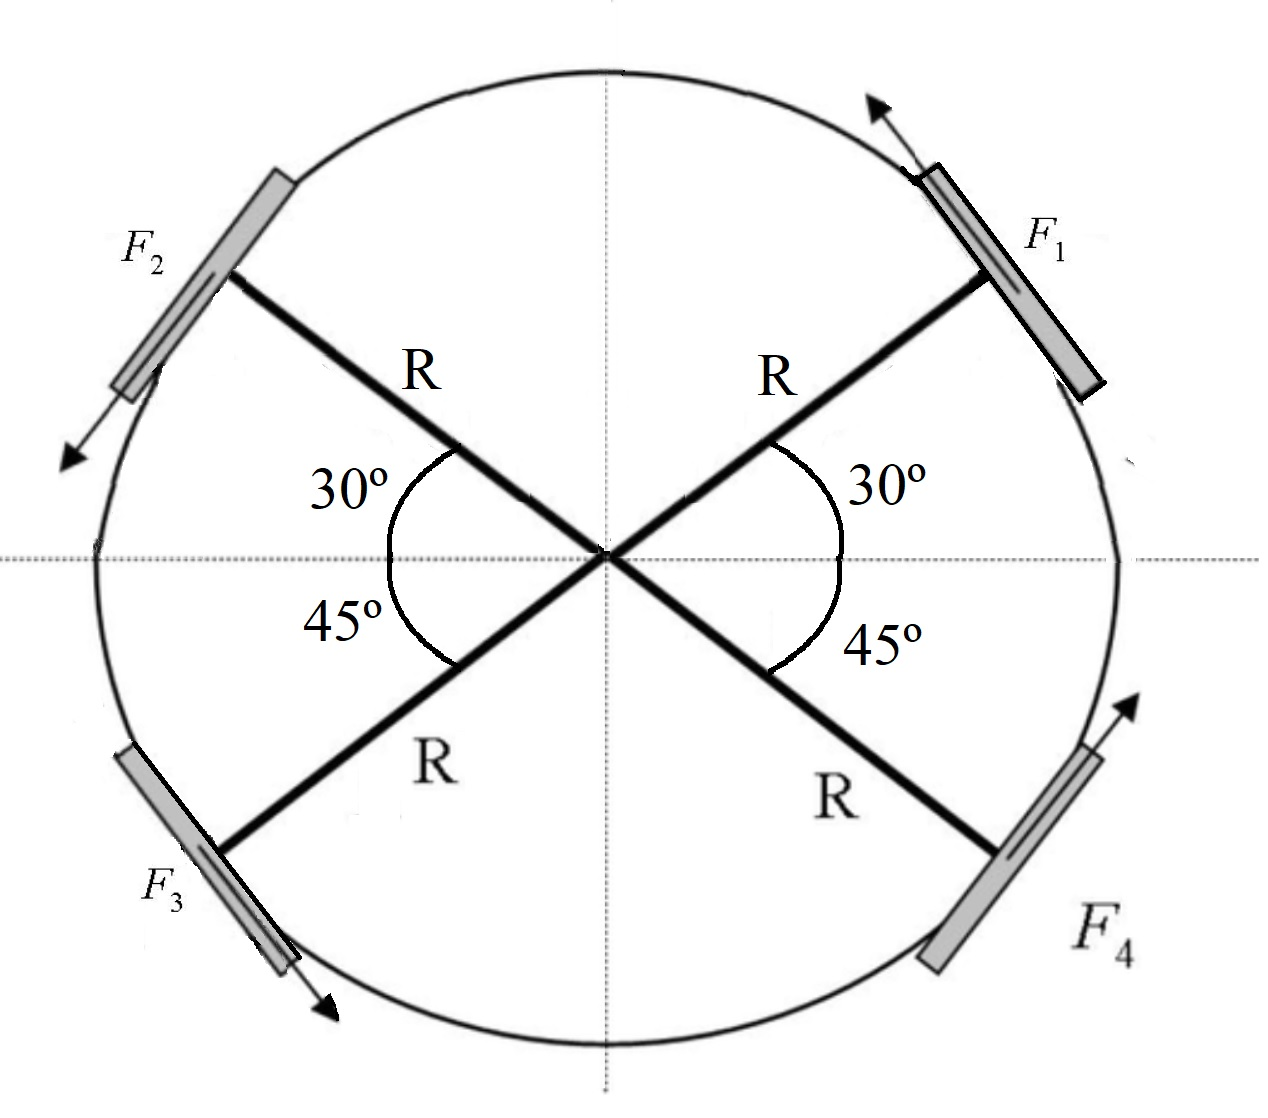
\includegraphics[width=0.4\textwidth]{sanhaco.jpg}
\caption{Geometria das rodas}
\label{Figura 1}
\end{figure}

Tem se que $m=\begin{pmatrix}v_{1},v_{2},v_{3},v_{4} \end{pmatrix}^T$ é o vetor em $\bkRsf^4$ da velocidade tangencial dos motores, $D$ é a matriz de acoplamento de velocidade, e $v$  é um vetor tridimensional $\begin{pmatrix}v_{x},v_{y},R{\omega}\ \end{pmatrix}^T$.
Dado a modelagem matemática do movimento do robô, discuta como um algoritmo pode ser criado para a identificação de velocidades inconsistentes entre os motores. Em outras palavras, crie um método para identificar o  deslizamento nas rodas do robô.

\subsection{Economia de Energia}

\hspace{1cm}Considerando o resultado do problema anterior, caso seja detectado uma roda deslizando, qual a influência do deslizamento no gasto energético do robô? Proponha uma correção adequada para as velocidades dos motores, de modo a corrigir o deslizamento e aumentar a eficiência energética da direção.

\section{Resolução do problema}
\subsection{Item 1}

\hspace{1cm}Consideremos o robô da figura, no qual os ângulos das rodas superiores são $\alpha=30^{\circ}$ e os da inferiores são $\beta=45^{\circ}$, o vetor $m = \begin{pmatrix} v_{1},v_{2},v_{3},v_{4} \end{pmatrix}^T$ representa as velocidades tangenciais dos motores e o vetor $v = \begin{pmatrix} v_{x},v_{y},Rw \end{pmatrix}^T$ a velocidade total do robô (translacional e rotacional).

Para procurarmos inconsistências nas velocidades dos motores (que indicam deslizamento nas rodas), partiremos da relação inicial dada por:
\[m = Dv\]
\[D
=
\begin{pmatrix}
  -\sin{\frac{\pi}{6}} &  \cos{\frac{\pi}{6}} & 1 \\
  -\sin{\frac{\pi}{6}} &  -\cos{\frac{\pi}{6}} &  1 \\
  \sin{\frac{\pi}{4}} & -\cos{\frac{\pi}{4}}   &  1  \\
  \sin{\frac{\pi}{4}} &  \cos{\frac{\pi}{4}} & 1
 \end{pmatrix}
\]
%%%%%%%%%%%%%%%%%%%%%%%%%%%%%%%%%

Como é possível notar, a matriz $D$ não é quadrada e, por tanto, não possui inversa. Assim não podemos, inicialmente, isolar o vetor $v$. No entanto, podemos calcular uma matriz, chamada Matriz Pseudoinversa ($D^+$), tal que $D^+D=I$ .Usaremos essa matriz com o intuito de isolar o vetor $v$.

\subsubsection{Definição Pseudo-inversa (Moore-Penrose)}

\hspace{1cm} A Pseudoinversa $D^+$ é definida como a matriz que satisfaz os quatro seguintes critérios (condições de Moore-Penrose):
\[DD^+D=D\]
\[D^+DD^+=D^+\]
\[(DD^+)^*=DD^+\]
\[(D^+D)^*=D^+D\]

No caso particular em que $D$ tem seu espaço coluna LI, podemos calcular a sua inversa da seguinte maneira:
\[ D^+ = (D^*D)^{-1} D^*\]

Assim, temos:

\[D^+
=
\begin{pmatrix}
  -0,4142    &-0,4142    & 0,4142    & 0,4142    \\
 0,3464 &  -0,3464 & -0,2828 & 0,2828 \\
 0,2929 & 0,2929 & 0,2071& 0,2071
 \end{pmatrix}
\]

\subsubsection{Demonstração da propriedade}

\hspace{1cm} Assim, usando a expressão anterior e multiplicando por $D$ pela direita, temos:
\[D^+D = (D^*D)^{-1}(D^*D) = I \Rightarrow D^+ \text{ é a inversa a esquerda de }D\]  

\subsubsection{Teste de velocidades inconsistentes}

\hspace{1cm} Aplicando a pseudo-inversa na equação inicial, obtemos:
\[ m = Dv \Rightarrow D^+m = D^+Dv \Rightarrow v = D^+m\]

Com a constante comunicação do robô e do controlador acerca da situação das velocidades dos motores, podemos sempre testar a inconsistência da matriz m, de modo que se as relações $m = Dv$ e $v = D^+m$ são válidas, então $m = DD^+m$ também o é. Assim, para testar a consistência das velocidades, basta testar a validade da seguinte expressão:
\[ m = DD^+m \Rightarrow (I - DD^+)m = 0\]

Temos que:
\[(I - DD^+)
=
\begin{pmatrix}
  0,2000    &-0,2000    & 0,2449    & -0,2449    \\
 -0,2000 &  0,2000 & -0,2449 & 0,2449 \\
 0,2449 & -0,2449 &  0,3000  & -0,3000 \\
 -0,2449 & 0,2449 & -0,3000  & 0,3000
 \end{pmatrix}
\]


Se $m$ for consistente, a igualdade ocorrerá. Caso não ocorra, podemos afirmar com certeza que pelo menos uma roda está com velocidade inconsistente e, portanto, deslizando. Existe, porém, a possibilidade de que múltiplas rodas também estejam deslizando em uma taxa que faça com que a relação permaneça válida, no entanto, isto é extremamente improvável.

Para $\alpha = \pi/6$ e $\beta = \pi/4$, teremos a seguinte relação:
\[0,2(v_1 - v_2) = 0,2449(v_4 - v_3)\]

Logo, se essa relação \textbf{não} for válida, teremos identificado que há deslizamento no movimento do robô.

\subsection{Item 2}

\hspace{1cm}Se detectarmos que $m$ não é consistente, então temos que uma ou mais rodas estão desperdiçando energia ao rodar em falso. Para entendermos esse desperdício de energia precisamos identificar como funciona o vetor aceleração do robô, dado por: $ a = C_{\alpha}f$.
\[C_{alpha}
=
\begin{pmatrix}
  -\sin{\frac{\pi}{6}} & -\sin{\frac{\pi}{6}} & \sin{\frac{\pi}{4}} & \sin{\frac{\pi}{4}} \\
  \cos{\frac{\pi}{6}} &  -\cos{\frac{\pi}{6}} &  -\cos{\frac{\pi}{4}} &  \cos{\frac{\pi}{4}} \\
 \frac{1}{\alpha} & \frac{1}{\alpha} &\frac{1}{\alpha} & \frac{1}{\alpha}
 \end{pmatrix}
\]

Partindo desse ponto, é fácil notar que existem combinações de forças dos motores que geram uma aceleração nula: $ a = 0 $. Temos como exemplo o vetor: $f_{o} = \begin{pmatrix} -\sqrt{\frac{2}{3}},\sqrt{\frac{2}{3}},-1,1\end{pmatrix}^T$. Em outras palavras, o vetor $f_{o}$ pertence ao núcleo de $C_{\alpha}$.

Essa interessante observação nos permite expandir o raciocínio para resolver o problema de desperdício de energia. Note que se um vetor $g$ pertence ao núcleo de $C_{\alpha}$, então qualquer combinação de vetores $f$ que inclua $g$ produz a mesma aceleração que $f - g$, pois:
\[ a = C_{\alpha}(f) = C_{\alpha}(f-g) + C_{\alpha}(g) = C_{\alpha}(f-g)\]

Assim, para uma aceleração $a$, existe uma única força tal que $f=C_{\alpha}^+a$. Como $f$ é sempre menor em módulo do que $f-g$ (porque $g$ é ortogonal ao subespaço de $f$), temos a situação onde gastasse menos energia. Conclui-se que os motores não desperdiçam energia quando forças do Núcleo de $C_{\alpha}$ são evitadas.

Como pode se verificar, $C_{alpha}$ possui 3 colunas LI. Assim, $dim(C_{alpha}) = 3$, daí, aplicando o teorema do posto-nulidade para $C_{\alpha}$, temos:
\[Rank(C_{\alpha}) + Ker(C_{\alpha}) = \text{ número de colunas de }C_{alpha}\]


Portanto $Ker(C_{\alpha}) = 1 $, e portanto qualquer vetor no núcleo de $C_{\alpha}$ é da forma $\lambda f_{k}$.

O fato interessante de se notar é que primeiro, testamos as validades das velocidades através da equação: $(I-DD^+)m = 0$ e agora, concluímos que qualquer vetor no núcleo de $C_{\alpha}$ gera uma aceleração nula no robô. Podemos estreitar ainda mais essa relação, se usarmos o conceito de operador de projeção ortogonal:

As matrizes $DD^+ e D^+D$ são operadores de projeção ortogonal, $P$ , ou seja, são hermitianos ($P = P^*$), por definição, e são idempotentes ($P^2 = P$). Daí, as seguintes propriedades se seguem:

$DD^+$ é o operador de projeção ortogonal na $Im(D)$, e por consequência, $I - DD^+$ é o operador de projeção ortogonal em $ker(D^*)$.
%%%%%%%%%%%
Se analisarmos as matrizes $C_{\alpha}$ e $D$, podemos notar que $C_{\alpha} = (1/{\alpha}M)(D^T)$, como nossas matrizes estão no corpo dos $\bkRsf$, sabemos que $D^T = D^*$, então podemos ver que $C_{\alpha}$ é a matriz adjunta de $D$ multiplicada por uma constante!

Então, concluimos que a transformação $(I-DD^+)$ projeta $m$ no $ker(D^*)$. Além disso, sabemos que $m$ é consistente se $(I-DD^+)m = 0$. Portanto, chegamos que $m$ é consistente se é ortogonal ao vetor que compõe a base do $ker(C_{\alpha})$.

\subsection{Correção do deslizamento}

\hspace{1cm} Do que foi mostrado anteriormente, concluimos também que as velocidades dos motores são inconsistentes se existe uma projeção de $m$ na direção do vetor $f_{o}$, que é base do espaço nulo de $C_{\alpha}$. Portanto, para corrigir o deslizamento, nós calcularemos a projeção de $m$ na direção do vetor unitário na direção de $f_{o}$ e subtrairemos essa projeção de $m$.

\[m_{corrigido} = m - (m . f_{o}^")f_{o}^" \text{ ,  onde } f_{o}^" \text{é o vetor unitário na direção de }f_{o} \]

Podemos visualizar a correção de deslizamento da seguinte maneira: o espaço vetorial de $m$ tem $\text{dimensão}= 4$. Nesse espaço, existe um subespaço tridimensional (um hiperplano tridimensional) de valores consistentes, ou seja, que não deslizam. Ortogonalmente à esse subespaço, possuímos o vetor $f_{o}$. Sempre que as rodas estão deslizando, estamos gastando energia, pois o vetor das velocidades contém uma componente na direção $f_{o}$.

Daí, a nossa correção para velocidades inconsistentes gera, consequentemente, uma economia de energia para o sistema do robô.

Além disso, quando mapeamos as acelerações Euclidianas $a$ com as forças dos motores $f$, sempre obtemos resultados consistentes, através da expressão:
\[f = C_{\alpha}^+a\]

Veja que $rank(C_{\alpha}) = 3$, então pelo teorema do posto-nulidade temos que: $ker(C_{\alpha}) = 0$. $C_{\alpha}$, portanto, mapeia as acelerações $a$  em $f$ com uma bijeção (subespaço de dimensão 3). Se esse espaço possuísse algum elemento $u$ do núcleo de $C_{\alpha}$, então deveria existir uma aceleração $a$, diferente de 0, tal que $u = C_{\alpha}^+a$. Como vimos anteriormente que $c_ {\alpha}u = a = 0$, chegaríamos a um absurdo.


\end{document}documentclass{article}

\usepackage{grapicx}
\usepackage[utf8]{inputenc}

\renewcommand*\contentsname{Sumário}
\begin{document}

\begin{figure}
    
\includegraphics[width=\linewidth]{ime.jpg}
\end{figure}

\tableofcontents
\newpage

\section{Introdução}

\section{Discussão do Problema}

\section{Resolução do Problema}

\section{Conclusão}

\end{document}